The evaluation of the algorithms performance was mainly done qualitatively.
For short camera trajectories the quality of the reconstruction was quite good.
For longer trajectories, however, the error tends to accumulate over time and the
probability to completely loose track of the motion increases.
This is understandable since the tracking on a noisy map introduces more noise
in the movement which in turn leads to even more noise in the newly reconstructed
part of the map.
Figure \ref{fig:tracking_error_reconstruction} shows the development of the error
in comparison to the total travelled distance over a trajectory with 140,000 timesteps.
We expect these results to improve with more carefully selected parameters for the
tracking and reconstruction.
An example for a result of the complete algorithm can be seen in figure \ref{fig:zigzag_reconstruction}.
Observing the different parts isolated shows even sub-pixel accuracy.
Reconstructing the scene with ground truth data for the camera orientations can produce sharp images
with even higher resolution than the input image. An example for the isolated reconstruction results
is shown in figure \ref{fig:reconstruction_only}.
In our experiments, tracking the camera motion with the input image as map consistently lead to a deviation
of the estimate to the ground truth of less than 1 pixel (figure \ref{fig:tracking_groundtruth}). The estimated track is, however, oscillating heavily
the ground truth what could lead to some noise in the reconstruction. We tried to tackle
this problem by using low-pass filters on the estimated positions, but did not manage to
adapt the parameters in a way to receive completely satisfying results.

Our additional experiments produced quite promising results.
By removing a shutter in front of the camera and simply integrating the events,
an image is produced that is easily identifiable as the recorded scene (figure \ref{fig:shutter_integration}).
It is, however, quite noisy and obviously suffers from the low resolution of the sensor.
We are still confident that the resulting image could be filtered in such a way that
a sufficiently clear image for the tracking can be received.
The images generated for calibration were also noisy (figure \ref{fig:calibration}), but could easily be used
for calibration with the Matlab camera calibration app without further filtering.

\begin{figure}
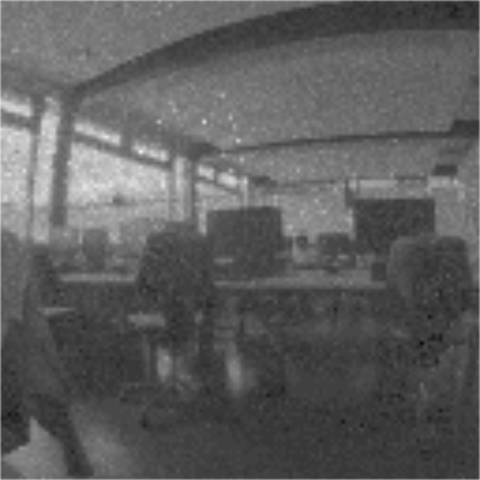
\includegraphics[width=\linewidth]{images/PCLab_integrated.png}
\caption{image of our lab generated by integrating over short interval while removing shutter}
\label{fig:shutter_integration}
\end{figure}

\begin{figure}
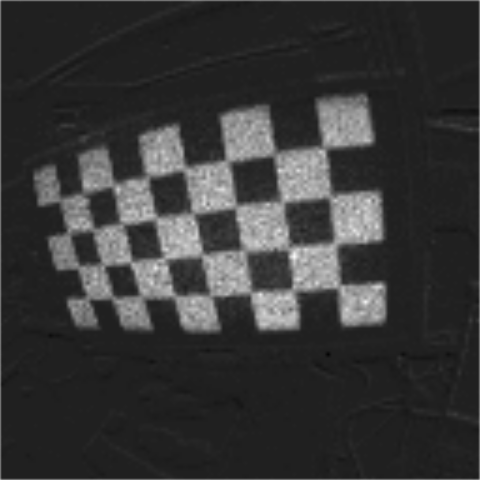
\includegraphics[width=\linewidth]{images/checkerboard_integrated.png}
\caption{a sample checkerboard pattern used for calibration}
\label{fig:calibration}
\end{figure}

\begin{figure}
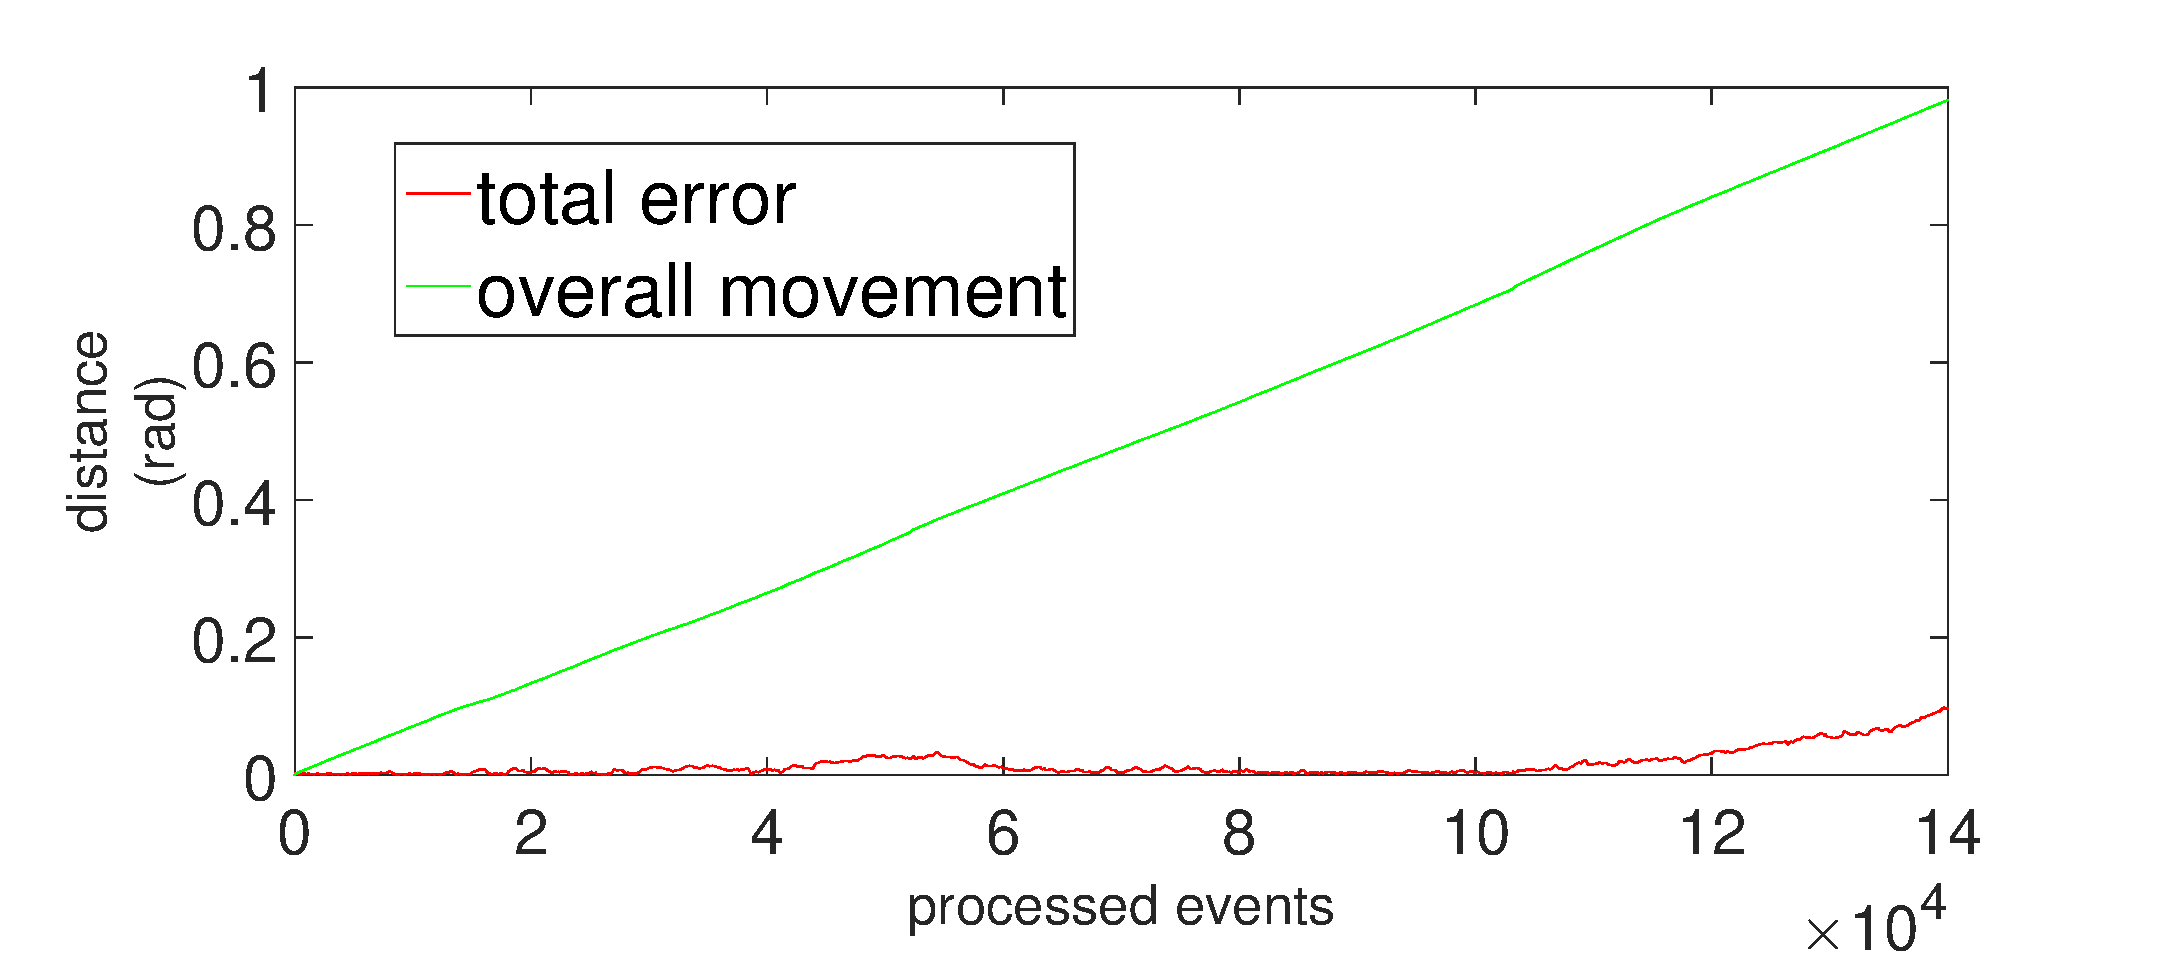
\includegraphics[width=\linewidth]{images/Tracking_error_during_reconstruction.eps}
\label{fig:tracking_error_reconstruction}
\caption{The tracking error (red) in comparison to the total travelled distance (green)
while reconstructing the map.
}
\end{figure}

\begin{figure}
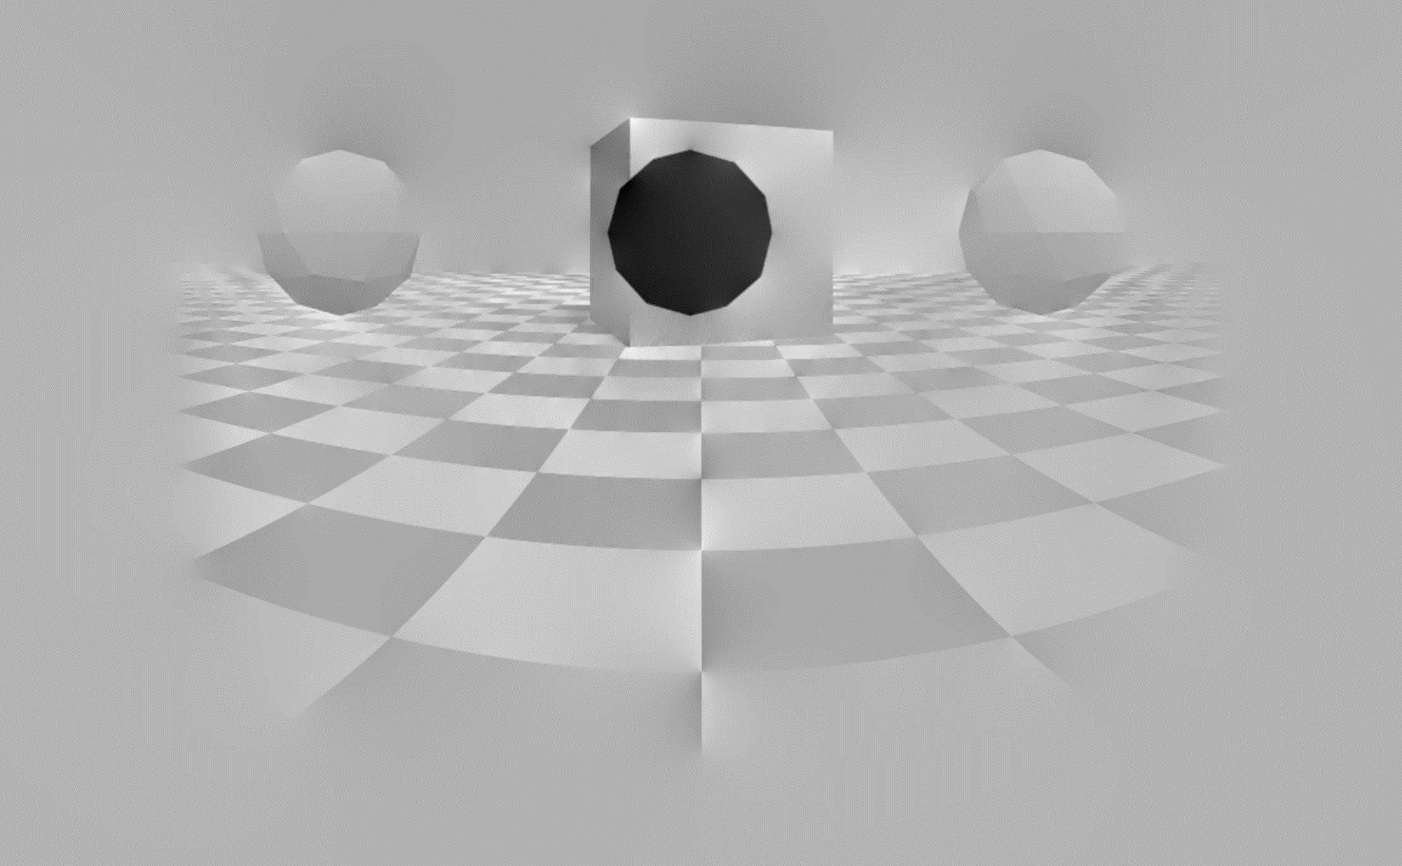
\includegraphics[width=\linewidth]{images/simulation_reconstruction.jpg}
\label{fig:reconstruction_only}
\caption{Reconstruction of the scene with ground truth data for the camera positions.}
\end{figure}

\begin{figure}
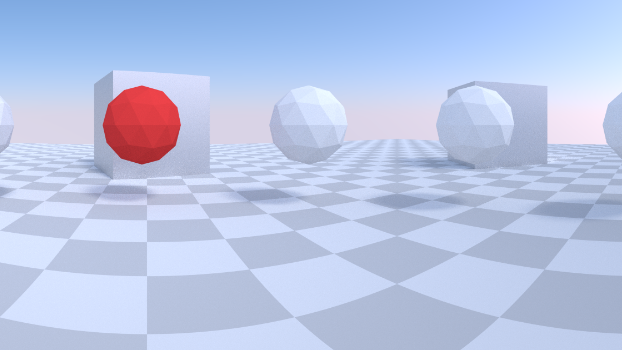
\includegraphics[width=\columnwidth]{images/zigzag_input.png}
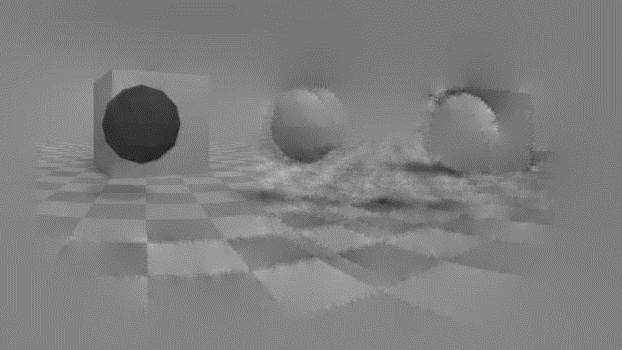
\includegraphics[width=\columnwidth]{images/zigzag_reconstruction.png}
\caption{A part of the input scene (top) and its reconstruction,
moving the camera in a large triangle waveform pattern to the right.
The area around the leftmost ball in the scene was used to initialize
the map as described in section \ref{sec:core_algorithm}.}
\label{fig:zigzag_reconstruction}
\end{figure}

\begin{figure}
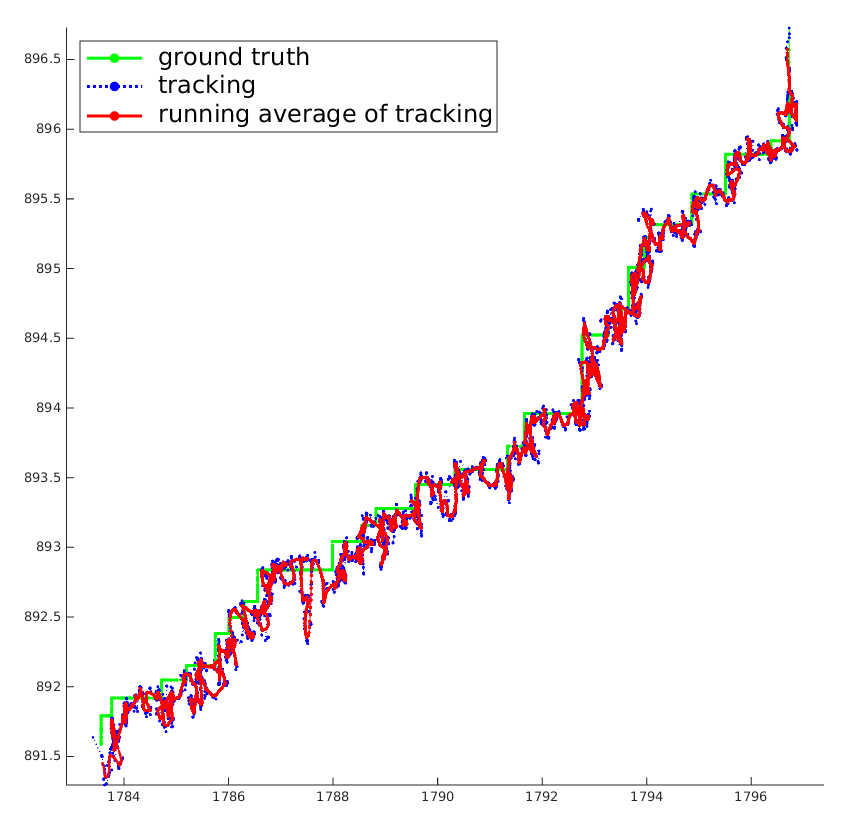
\includegraphics[width=\columnwidth]{images/tracking_without_reconstruction.png}
\caption{tracking with ground truth data, i.e. without image reconstruction}
\label{fig:tracking_groundtruth}
\end{figure}
